% answers.tex —— 1994 年·上海试点教材文科卷 · 参考答案与详细解析片段
% 由 tools/generate_projects.py 依来源总账自 1994/1994_数学真题_上海试点文_试题.md + 1994/1994_数学真题_上海试点文_解析正文.md + 1994/1994_数学真题_上海试点文_答案要点.md 生成，勿手改（改源 MD 后重跑）


\begin{gktip}
下列过程按指定 PDF 题后所载解答和累计评分点整理；发布主体、出版者、版次及答案官方性未核实。原页说明第 21–26 题右端分数表示做到该步的累计分数。
\end{gktip}

\gkpart{一、填空题与选择题}

\begin{answer}
\gksolhead{1}{填空题}

\textbf{题目}：

不等式 $|x+1|<1$ 的解是\gkblank{}。

\Needspace{4\baselineskip}
\textbf{解析}

卷内仅列答案，无推导。

\gkanswer{答案：$-2<x<0$}

\end{answer}
\begin{answer}
\gksolhead{2}{填空题}

\textbf{题目}：

函数 $y=\sin^2 x$ 的最小正周期是\gkblank{}。

\Needspace{4\baselineskip}
\textbf{解析}

卷内仅列答案，无推导。

\gkanswer{答案：$\pi$}

\end{answer}
\begin{answer}
\gksolhead{3}{填空题}

\textbf{题目}：

计算：$\displaystyle\lim_{x\to-1}\frac{x^2-2x-3}{x+1}=$\gkblank{}。

\Needspace{4\baselineskip}
\textbf{解析}

卷内仅列答案，无推导。

\gkanswer{答案：$-4$}

\end{answer}
\begin{answer}
\gksolhead{4}{填空题}

\textbf{题目}：

以点 $C(-2,3)$ 为圆心且与 $y$ 轴相切的圆的方程是\gkblank{}。

\Needspace{4\baselineskip}
\textbf{解析}

卷内仅列答案，无推导。

\gkanswer{答案：$(x+2)^2+(y-3)^2=4$}

\end{answer}
\begin{answer}
\gksolhead{5}{填空题}

\textbf{题目}：

方程 $\log_3(x-1)=\log_9(x+5)$ 的解是\gkblank{}。

\Needspace{4\baselineskip}
\textbf{解析}

卷内仅列答案，无推导。

\gkanswer{答案：$x=4$}

\end{answer}
\begin{answer}
\gksolhead{6}{填空题}

\textbf{题目}：

函数 $y=\sqrt{x^2-1}\ (x\le -1)$ 的反函数是\gkblank{}。

\Needspace{4\baselineskip}
\textbf{解析}

卷内仅列答案，无推导。

\gkanswer{答案：$y=-\sqrt{x^2+1}\ (x\ge0)$}

\end{answer}
\begin{answer}
\gksolhead{7}{填空题}

\textbf{题目}：

双曲线 $\dfrac{y^2}{2}-x^2=1$ 的两个焦点的坐标是\gkblank{}。

\Needspace{4\baselineskip}
\textbf{解析}

卷内仅列答案，无推导。

\gkanswer{答案：$(0,\sqrt3)$ 和 $(0,-\sqrt3)$}

\end{answer}
\begin{answer}
\gksolhead{8}{填空题}

\textbf{题目}：

$\left(x^3-\dfrac{2}{x^2}\right)^5$ 的展开式中 $x^5$ 的系数是\gkblank{}（结果用数值表示）。

\Needspace{4\baselineskip}
\textbf{解析}

卷内仅列答案，无推导。

\gkanswer{答案：$40$}

\end{answer}
\begin{answer}
\gksolhead{9}{填空题}

\textbf{题目}：

如果复数 $\dfrac{2+bi}{1-2i}$（其中 $i$ 为虚数单位，$b$ 为实数）的实部和虚部相等，那么 $b=$\gkblank{}。

\Needspace{4\baselineskip}
\textbf{解析}

卷内仅列答案，无推导。

\gkanswer{答案：$-\dfrac23$}

\end{answer}
\begin{answer}
\gksolhead{10}{填空题}

\textbf{题目}：

某商场计划经销某种商品，预测可得盈利 30000 元、26000 元、8000 元的概率分别为 0.3、0.6、0.1，则经销该商品的期望盈利为\gkblank{}元。

\Needspace{4\baselineskip}
\textbf{解析}

卷内仅列答案，无推导。

\gkanswer{答案：$25400$}

\end{answer}
\begin{answer}
\gksolhead{11}{选择题}

\textbf{题目}：

当 $a>1$ 时，函数 $y=\log_a x$ 和 $y=(1-a)x$ 的图象只可能是\mbox{（　　）}。

（A）递增直线过原点，递增对数曲线过 $(1,0)$；（B）递减直线过原点，递增对数曲线过 $(1,0)$；（C）递增直线过原点，递减对数曲线过 $(1,0)$；（D）递减直线过原点，递减对数曲线过 $(1,0)$。（原卷各选项为函数图象。）
\nopagebreak[4]
\begin{center}% 依试点教材文科固定来源第 1 页四种函数图象选项转绘；拓扑示意，不表示精确比例。
\begin{center}
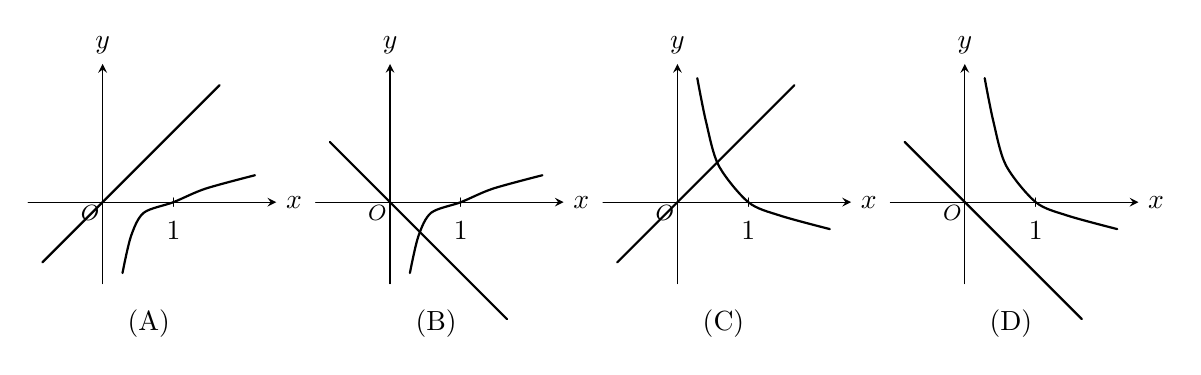
\begin{tikzpicture}[x=0.9cm,y=0.9cm,>=stealth,line cap=round,line join=round]
\foreach \xshift/\label/\lineup/\logup in {0/A/1/1,3.65/B/-1/1,7.3/C/1/-1,10.95/D/-1/-1} {
  \begin{scope}[xshift=\xshift cm]
    \draw[->] (-1.05,0)--(2.45,0) node[right] {$x$};
    \draw[->] (0,-1.15)--(0,1.95) node[above] {$y$};
    \draw (1,0.06)--(1,-0.06) node[below=2pt] {$1$};
    \node[below left,font=\footnotesize,inner sep=1pt] at (0,0) {$O$};
    \ifnum\lineup=1
      \draw[thick] (-0.85,-0.85)--(1.65,1.65);
    \else
      \draw[thick] (-0.85,0.85)--(1.65,-1.65);
    \fi
    \ifnum\logup=1
      \draw[thick] plot[smooth] coordinates {(0.28,-1.0) (0.4,-0.48) (0.58,-0.15) (1,0) (1.45,0.19) (2.15,0.38)};
    \else
      \draw[thick] plot[smooth] coordinates {(0.28,1.75) (0.4,1.15) (0.58,0.52) (1,0) (1.45,-0.19) (2.15,-0.38)};
    \fi
    \node[below] at (0.65,-1.38) {(\label)};
  \end{scope}
}
\end{tikzpicture}
\end{center}
\end{center}
\nopagebreak[4]
\Needspace{4\baselineskip}
\textbf{解析}

卷内仅列答案，无推导。

\gkanswer{答案：B}

\end{answer}
\begin{answer}
\gksolhead{12}{选择题}

\textbf{题目}：

如果 $0<a<1$，那么下列不等式中正确的是\mbox{（　　）}。

（A）$(1-a)^{1/3}>(1-a)^{1/2}$　（B）$\log_{1-a}(1+a)>0$

（C）$(1-a)^3>(1+a)^2$　（D）$(1-a)^{1+a}>1$

\Needspace{4\baselineskip}
\textbf{解析}

卷内仅列答案，无推导。

\gkanswer{答案：A}

\end{answer}
\begin{answer}
\gksolhead{13}{选择题}

\textbf{题目}：

已知直线 $2x+y-2=0$ 和 $mx-y+1=0$ 的夹角为 $\dfrac\pi4$，那么 $m$ 的值为\mbox{（　　）}。

\begin{gkopts}(2)
\task （A）$-\dfrac13$ 或 $-3$
\task （B）$\dfrac13$ 或 $3$
\task （C）$-\dfrac13$ 或 $3$
\task （D）$\dfrac13$ 或 $-3$
\end{gkopts}

\Needspace{4\baselineskip}
\textbf{解析}

卷内仅列答案，无推导。

\gkanswer{答案：C}

\end{answer}
\begin{answer}
\gksolhead{14}{选择题}

\textbf{题目}：

已知 $a,b$ 是异面直线，直线 $c$ 平行于直线 $a$，那么 $c$ 与 $b$\mbox{（　　）}。

\begin{gkopts}(2)
\task （A）一定是异面直线
\task （B）一定是相交直线
\task （C）不可能是平行直线
\task （D）不可能是相交直线
\end{gkopts}

\Needspace{4\baselineskip}
\textbf{解析}

卷内仅列答案，无推导。

\gkanswer{答案：C}

\end{answer}
\begin{answer}
\gksolhead{15}{选择题}

\textbf{题目}：

设 $I$ 是全集，集合 $P,Q$ 满足 $P\subset Q$，则下面的结论中错误的是\mbox{（　　）}。

\begin{gkopts}(2)
\task （A）$P\cup Q=Q$
\task （B）$\overline P\cup Q=I$
\task （C）$P\cap\overline Q=\varnothing$
\task （D）$\overline P\cap\overline Q=\overline P$
\end{gkopts}

\Needspace{4\baselineskip}
\textbf{解析}

卷内仅列答案，无推导。

\gkanswer{答案：D}

\end{answer}
\begin{answer}
\gksolhead{16}{选择题}

\textbf{题目}：

已知 $y=f(x)\ (x\in\mathbb R)$ 是奇函数，$f(5)\ne0$，则下列各点中，在 $y=f(x)$ 的图象上的点是\mbox{（　　）}。

\begin{gkopts}(4)
\task （A）$(5,f(-5))$
\task （B）$(-5,-f(5))$
\task （C）$(-5,f(5))$
\task （D）$(5,-f(5))$
\end{gkopts}

\Needspace{4\baselineskip}
\textbf{解析}

卷内仅列答案，无推导。

\gkanswer{答案：B}

\end{answer}
\begin{answer}
\gksolhead{17}{选择题}

\textbf{题目}：

设 $a,b$ 是平面 $\alpha$ 外的任意两条线段，则“$a,b$ 的长相等”是“$a,b$ 在平面 $\alpha$ 内的射影长相等”的\mbox{（　　）}。

\begin{gkopts}(2)
\task （A）非充分条件也非必要条件
\task （B）充分必要条件
\task （C）必要条件而非充分条件
\task （D）充分条件而非必要条件
\end{gkopts}

\Needspace{4\baselineskip}
\textbf{解析}

卷内仅列答案，无推导。

\gkanswer{答案：A}

\end{answer}
\begin{answer}
\gksolhead{18}{选择题}

\textbf{题目}：

9 支足球队中，有 5 支亚洲队、4 支非洲队，从中任意抽取两队进行比赛，则 1 队是亚洲队且 1 队是非洲队的概率是\mbox{（　　）}。

\begin{gkopts}(2)
\task （A）$\dfrac{C_5^1+C_4^1}{C_9^2}$
\task （B）$\dfrac{C_4^1}{C_9^2}$
\task （C）$\dfrac{C_5^2}{C_9^2}$
\task （D）$\dfrac{C_5^1C_4^1}{C_9^2}$
\end{gkopts}

\Needspace{4\baselineskip}
\textbf{解析}

卷内仅列答案，无推导。

\gkanswer{答案：D}

\end{answer}
\begin{answer}
\gksolhead{19}{选择题}

\textbf{题目}：

在直角坐标系 $xOy$ 中，曲线 $C$ 的方程是 $y=\cos x$，现平移坐标系，把原点移到点 $O'\left(\dfrac\pi2,-\dfrac\pi2\right)$，则在坐标系 $x'O'y'$ 中，曲线 $C$ 的方程是\mbox{（　　）}。

\begin{gkopts}(2)
\task （A）$y'=\sin x'+\dfrac\pi2$
\task （B）$y'=-\sin x'+\dfrac\pi2$
\task （C）$y'=\sin x'-\dfrac\pi2$
\task （D）$y'=-\sin x'-\dfrac\pi2$
\end{gkopts}

\Needspace{4\baselineskip}
\textbf{解析}

卷内仅列答案，无推导。

\gkanswer{答案：B}

\end{answer}
\begin{answer}
\gksolhead{20}{选择题}

\textbf{题目}：

某个命题与自然数 $n$ 有关。如果当 $n=k\ (k\in\mathbb N)$ 时该命题成立，那么可推得当 $n=k+1$ 时该命题也成立。现已知当 $n=5$ 时该命题不成立，那么可推得\mbox{（　　）}。

\begin{gkopts}(2)
\task （A）当 $n=6$ 时该命题不成立
\task （B）当 $n=6$ 时该命题成立
\task （C）当 $n=4$ 时该命题不成立
\task （D）当 $n=4$ 时该命题成立
\end{gkopts}

\Needspace{4\baselineskip}
\textbf{解析}

卷内仅列答案，无推导。

\gkanswer{答案：C}

\end{answer}
\gkpart{三、解答题}

\begin{answer}
\gksolhead{21}{三角函数（12 分）}

\textbf{题目}（本题满分 12 分）：

已知 $\sin\alpha=\dfrac35$，$\alpha\in\left(\dfrac\pi2,\pi\right)$，$\tan(\pi-\beta)=\dfrac12$，求 $\tan(\alpha-2\beta)$ 的值。

\Needspace{4\baselineskip}
\textbf{解析}

\Needspace{5\baselineskip}
由 $\sin\alpha=\dfrac35$ 且 $\alpha\in(\dfrac\pi2,\pi)$，得
\nopagebreak[4]
\[
\cos\alpha=-\frac45,\qquad \tan\alpha=-\frac34.
\]
\Needspace{5\baselineskip}
又 $\tan(\pi-\beta)=\dfrac12$，故 $\tan\beta=-\dfrac12$，于是
\nopagebreak[4]
\[
\tan2\beta=\frac{2\tan\beta}{1-\tan^2\beta}
=\frac{2(-1/2)}{1-(-1/2)^2}=-\frac43.
\]
\Needspace{5\baselineskip}
因此
\nopagebreak[4]
\[
\tan(\alpha-2\beta)=\frac{\tan\alpha-\tan2\beta}{1+\tan\alpha\tan2\beta}
=\frac{-\frac34+\frac43}{1+\frac34\cdot\frac43}=\frac7{24}.
\]

卷内累计给分：由条件求出 $\cos\alpha,\tan\alpha$ 得 4 分；求出 $\tan2\beta$ 得 8 分；求出所求值得 12 分。

\gkanswer{答案：$\tan(\alpha-2\beta)=\dfrac7{24}$}

\end{answer}
\begin{answer}
\gksolhead{22}{空间向量（12 分）}

\textbf{题目}（本题满分 12 分）：

本题共有 2 个小题，第 1 小题满分 7 分，第 2 小题满分 5 分。

已知空间三个点 $P(-2,0,2)$、$Q(-1,1,2)$ 和 $R(-3,0,4)$。设 $\vec a=\overrightarrow{PQ}$，$\vec b=\overrightarrow{PR}$。

（1） 求 $\vec a$ 与 $\vec b$ 的夹角 $\theta$（用反三角函数表示）；

（2） 试确定实数 $k$，使 $k\vec a+\vec b$ 与 $k\vec a-2\vec b$ 互相垂直。

\Needspace{4\baselineskip}
\textbf{解析}

\gksubpart{(1) 夹角}

\nopagebreak[4]
\[
\vec a=\overrightarrow{PQ}=(1,1,0),\qquad
\vec b=\overrightarrow{PR}=(-1,0,2),
\]
\Needspace{5\baselineskip}
所以 $|\vec a|=\sqrt2$、$|\vec b|=\sqrt5$，且 $\vec a\cdot\vec b=-1$。于是
\nopagebreak[4]
\[
\cos\theta=\frac{\vec a\cdot\vec b}{|\vec a||\vec b|}
=-\frac{\sqrt{10}}{10},\qquad
\theta=\arccos\left(-\frac{\sqrt{10}}{10}\right).
\]
卷内累计给分：写出两向量得 2 分；写出模长得 4 分；求出夹角得 7 分。

\gksubpart{(2) 垂直条件}

\nopagebreak[4]
\[
(k\vec a+\vec b)\cdot(k\vec a-2\vec b)
=(k-1,k,2)\cdot(k+2,k,-4)
=2k^2+k-10.
\]
由垂直条件得 $2k^2+k-10=0$，故 $k=-\dfrac52$ 或 $k=2$。卷内累计给分：列出点积表达式得 9 分；解得两根得 12 分。

\gkanswer{答案（1）：$\theta=\arccos\left(-\dfrac{\sqrt{10}}{10}\right)$}

\gkanswer{答案（2）：$k=-\dfrac52$ 或 $k=2$}

\end{answer}
\begin{answer}
\gksolhead{23}{空间几何（12 分）}

\textbf{题目}（本题满分 12 分）：

本题共有 2 个小题，第 1 小题满分 6 分，第 2 小题满分 6 分。

如图，在梯形 $ABCD$ 中，$AD\parallel BC$，$\angle ABC=\dfrac\pi2$，$AB=a$，$AD=3a$，且 $\angle ADC=\arcsin\dfrac{\sqrt5}{5}$，又 $PA\perp$ 平面 $ABCD$，$PA=a$。求：

（1） 二面角 $P-CD-A$ 的大小（用反三角函数表示）；

（2） 点 $A$ 到平面 $PBC$ 的距离。
\nopagebreak[4]
\begin{center}% 依试点教材文科固定来源 PDF 第 3 页转绘梯形与棱锥的拓扑关系；不表示精确比例。
\begin{center}
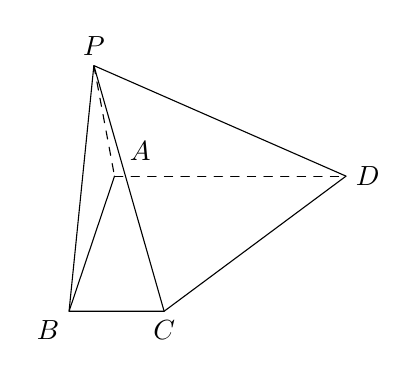
\begin{tikzpicture}[x=1.05cm,y=0.78cm,>=stealth,line cap=round,line join=round]
  \coordinate (B) at (0,0);
  \coordinate (A) at (0.55,2.2);
  \coordinate (C) at (1.15,0);
  \coordinate (D) at (3.35,2.2);
  \coordinate (P) at (0.3,4.0);
  \draw (A)--(B)--(C)--(D);
  \draw[dashed] (A)--(D);
  \draw (P)--(B) (P)--(C) (P)--(D);
  \draw[dashed] (P)--(A);
  \node[above right,xshift=2pt,yshift=2pt] at (A) {$A$};
  \node[below left] at (B) {$B$};
  \node[below] at (C) {$C$};
  \node[right] at (D) {$D$};
  \node[above] at (P) {$P$};
\end{tikzpicture}
\end{center}
\end{center}
\nopagebreak[4]
\Needspace{4\baselineskip}
\textbf{解析}

\gksubpart{(1) 二面角}

在平面 $ABCD$ 内过 $A$ 作 $AE\perp CD$，垂足为 $E$，连接 $PE$。因 $PA\perp$ 平面 $ABCD$，由三垂线定理得 $PE\perp CD$，所以 $\angle PEA$ 是二面角 $P-CD-A$ 的平面角。

\Needspace{5\baselineskip}
在直角三角形 $AED$ 中，$AD=3a$、$\angle ADE=\arcsin\dfrac{\sqrt5}{5}$，故
\nopagebreak[4]
\[
AE=AD\sin\angle ADE=\frac{3\sqrt5}{5}a.
\]
\Needspace{5\baselineskip}
在直角三角形 $PAE$ 中，按 350dpi 原页确认 $PA=a$，于是
\nopagebreak[4]
\[
\tan\angle PEA=\frac{PA}{AE}=\frac{\sqrt5}{3},
\]
故二面角大小为 $\arctan\dfrac{\sqrt5}{3}$。卷内累计给分：构造平面角得 2 分；求 $AE$ 得 4 分；求二面角得 6 分。

\gksubpart{(2) 点到平面的距离}

在平面 $PAB$ 内过 $A$ 作 $AH\perp PB$，垂足为 $H$。由 $PA\perp$ 平面 $ABCD$ 得 $PA\perp EC$；又 $AB\perp BC$，故 $BC\perp$ 平面 $PAB$，从而 $BC\perp AH$。因此 $AH\perp$ 平面 $PBC$，所求距离为 $AH$。

\Needspace{5\baselineskip}
在等腰直角三角形 $PAB$ 中，卷内给出
\nopagebreak[4]
\[
AH=\frac{\sqrt2}{2}a,
\]
所以点 $A$ 到平面 $PBC$ 的距离是 $\dfrac{\sqrt2}{2}a$。卷内累计给分依次为 8、10、12 分；并注明图中点 $E$ 若画在线段 $CD$ 内，不扣分。

\gkanswer{答案（1）：二面角 $P-CD-A$ 的大小为 $\arctan\dfrac{\sqrt5}{3}$（卷内记作 $\operatorname{arctg}\dfrac{\sqrt5}{3}$）}

\gkanswer{答案（2）：点 $A$ 到平面 $PBC$ 的距离为 $\dfrac{\sqrt2}{2}a$}

\end{answer}
\gkpart{四、解答题}

\begin{answer}
\gksolhead{24}{抛物线与垂直平分线（16 分）}

\textbf{题目}（本题满分 16 分）：

本题共有 2 个小题，第 1 小题满分 6 分，第 2 小题满分 10 分。

如图，抛物线 $y=3x^2$ 和 $y=-x^2+4ax\ (a>0)$ 交于原点 $O$ 和点 $A$。

（1） 求这两条抛物线所围成的图形的面积；

（2） 过点 $A$ 作抛物线 $y=-x^2+4ax$ 的切线，该切线与抛物线 $y=3x^2$ 交于另一点 $P$，求线段 $AP$ 的垂直平分线的方程。
\nopagebreak[4]
\begin{center}% 由固定来源示意图按 a=1（或 t=1）重绘；保留两抛物线、公共交点 O/A 与 A 点切线的拓扑关系。
\begin{center}
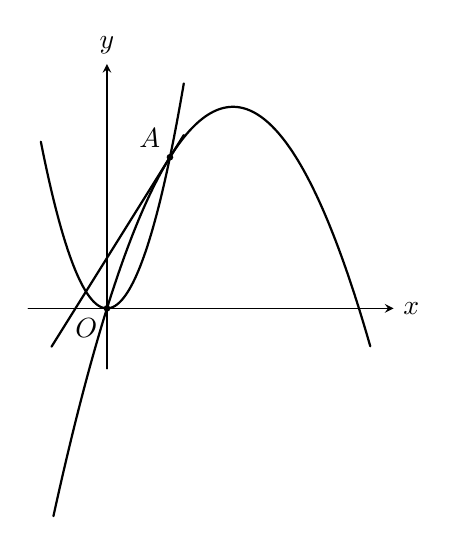
\begin{tikzpicture}[x=0.8cm,y=0.64cm,>=stealth,line cap=round,line join=round]
  \draw[->] (-1.25,0)--(4.55,0) node[right] {$x$};
  \draw[->] (0,-1.2)--(0,4.85) node[above] {$y$};
  \draw[thick,domain=-1.05:1.22,samples=80] plot (\x,{3*\x*\x});
  \draw[thick,domain=-0.85:4.18,samples=120] plot (\x,{-\x*\x+4*\x});
  \draw[thick] (-0.88,-0.76)--(1.22,3.44);
  \fill (0,0) circle (1.2pt);
  \fill (1,3) circle (1.2pt);
  \node[below left] at (0,0) {$O$};
  \node[above left] at (1,3) {$A$};
\end{tikzpicture}
\end{center}
\end{center}
\nopagebreak[4]
\Needspace{4\baselineskip}
\textbf{解析}

\gksubpart{(1) 围成图形的面积}

\Needspace{5\baselineskip}
联立 $y=3x^2$ 与 $y=-x^2+4ax$，交点横坐标为 $0,a$，故 $A=(a,3a^2)$。两曲线围成面积
\nopagebreak[4]
\[
S=\int_0^a\bigl((-x^2+4ax)-3x^2\bigr)\,dx
=\left(-\frac43x^3+2ax^2\right)_0^a=\frac23a^3.
\]
卷内累计给分：求出 $A$ 坐标得 2 分；列积分并求面积得 6 分。

\gksubpart{(2) 垂直平分线}

\Needspace{5\baselineskip}
曲线 $y=-x^2+4ax$ 的导数为 $y'=-2x+4a$，故点 $A$ 处切线斜率为 $2a$，切线方程为 $y=2ax+a^2$。与 $y=3x^2$ 联立，除 $A$ 外交点为
\nopagebreak[4]
\[
P=\left(-\frac a3,\frac{a^2}{3}\right).
\]
\Needspace{5\baselineskip}
$AP$ 中点为 $M=(\dfrac a3,\dfrac53a^2)$，且 $AP$ 斜率为 $2a$，故垂直平分线斜率为 $-\dfrac1{2a}$。代入点斜式得
\nopagebreak[4]
\[
y=-\frac1{2a}\left(x-\frac a3\right)+\frac53a^2
=-\frac1{2a}x+\frac53a^2+\frac16.
\]
卷内累计给分：求切线方程得 10 分；求出 $P$ 得 12 分；求中点得 14 分；写出垂直平分线得 16 分。

\gkanswer{答案（1）：$\dfrac23a^3$}

\gkanswer{答案（2）：$y=-\dfrac1{2a}x+\dfrac53a^2+\dfrac16$}

\end{answer}
\begin{answer}
\gksolhead{25}{数列（18 分）}

\textbf{题目}（本题满分 18 分）：

本题共有 3 个小题，第 1 小题满分 6 分，第 2 小题满分 6 分，第 3 小题满分 6 分。

设 $\{a_n\}$ 是公差为 $d$ 的等差数列，$a_3+a_5=2$，$S_{20}=a_1+a_2+\cdots+a_{20}=150$，又 $b_n=2^{a_n-2a_{n+1}}\ (n\in\mathbb N)$。

（1） 求 $a_1,d$ 的值；

（2） 求证 $\{b_n\}$ 是等比数列，并求 $b_n$；

（3） 设 $k$ 为某个自然数，且满足 $\displaystyle\lim_{n\to\infty}(b_kb_{k+1}+b_{k+1}b_{k+2}+\cdots+b_nb_{n+1})=\dfrac1{96}$，求 $k$ 的值。

\Needspace{4\baselineskip}
\textbf{解析}

\gksubpart{(1) 求 $a_1,d$}

\Needspace{5\baselineskip}
由等差数列条件，
\nopagebreak[4]
\[
a_3+a_5=2\Rightarrow 2a_1+6d=2,
\]
\nopagebreak[4]
\[
S_{20}=\frac{20(a_1+a_{20})}{2}=150
\Rightarrow 10(2a_1+19d)=150.
\]
解得 $a_1=-2,d=1$。卷内累计给分：列出方程组得 4 分；解得数值得 6 分。

\gksubpart{(2) 等比数列 $\{b_n\}$}

\nopagebreak[4]
\[
b_n=2^{a_n-2a_{n+1}},\qquad b_{n+1}=2^{a_{n+1}-2a_{n+2}},
\]
\Needspace{5\baselineskip}
所以
\nopagebreak[4]
\[
\frac{b_{n+1}}{b_n}=2^{3a_{n+1}-2a_{n+2}-a_n}=2^{-d}=\frac12.
\]
\Needspace{5\baselineskip}
故 $\{b_n\}$ 是等比数列。又 $b_1=1$，因此
\nopagebreak[4]
\[
b_n=\left(\frac12\right)^{n-1}.
\]
卷内累计给分：列出相邻项并化为指数得 8 分；说明公比为 $\frac12$ 得 10 分；求得通项得 12 分。

\gksubpart{(3) 极限条件}

\Needspace{5\baselineskip}
由（2），$b_kb_{k+1}=(\dfrac12)^{2k-1}$，且后续相邻乘积构成首项为 $(\dfrac12)^{2k-1}$、公比为 $(\dfrac12)^2$ 的等比数列。于是
\nopagebreak[4]
\[
\lim_{n\to\infty}\sum_{j=k}^{n}b_jb_{j+1}
=\frac{(\frac12)^{2k-1}}{1-(\frac12)^2}
=\frac{8}{3\cdot2^{2k}}=\frac1{96}.
\]
得 $2^{2k}=2^8$，所以 $k=4$。卷内累计给分：识别该等比数列得 15 分；求得 $k$ 得 18 分。

\gkanswer{答案（1）：$a_1=-2,\ d=1$}

\gkanswer{答案（2）：$\{b_n\}$ 是等比数列，$b_n=\left(\dfrac12\right)^{n-1}$}

\gkanswer{答案（3）：$k=4$}

\end{answer}
\begin{answer}
\gksolhead{26}{向量变换、面积与单调性（20 分）}

\textbf{题目}（本题满分 20 分）：

本题共有 3 个小题，第 1 小题满分 4 分，第 2 小题满分 10 分，第 3 小题满分 6 分。

设 $P(1,t)$ 是直角坐标系内的点（$t>0$）。将向量 $\overrightarrow{OP}$ 绕原点 $O$ 按逆时针方向旋转 $\dfrac\pi2$，再把它的模变为原来的两倍，得到向量 $\overrightarrow{OQ}$，以 $OP$、$OQ$ 为邻边作矩形 $OPRQ$。

（1） 求点 $Q,R$ 的坐标；

（2） 求矩形 $OPRQ$ 在第一象限部分的面积 $S(t)$；

（3） 确定函数 $S(t)$ 的单调区间，并加以证明。

\Needspace{4\baselineskip}
\textbf{解析}

\gksubpart{(1) 坐标}

\Needspace{5\baselineskip}
$\overrightarrow{OP}=(1,t)$。旋转 $\dfrac\pi2$ 后方向为 $(-t,1)$，再将模长变为原来的两倍，故
\nopagebreak[4]
\[
\overrightarrow{OQ}=\pm2(-t,1).
\]
由题意点 $Q$ 在第二象限，取 $\overrightarrow{OQ}=(-2t,2)$，于是 $Q=(-2t,2)$。又 $\overrightarrow{OR}=\overrightarrow{OP}+\overrightarrow{OQ}$，所以 $R=(1-2t,t+2)$。卷内累计给分至此为 4 分。

\gksubpart{(2) 面积分段}

\Needspace{5\baselineskip}
当 $0<t<\dfrac12$ 时，$R$ 在第一象限，矩形位于第一象限的部分是四边形 $OPRK$。直线 $QR$ 方程为 $y-2=t(x+2)$，令 $x=0$ 得 $K=(0,2t^2+2)$。按卷内面积分割，
\nopagebreak[4]
\[
S_{OPRK}=S_{OPRQ}-S_{OKQ}
=2(\sqrt{1+t^2})^2-\frac12(2t^2+2)\cdot2t
=2(1-t+t^2-t^3).
\]
\Needspace{5\baselineskip}
当 $t\ge\dfrac12$ 时，$R$ 在 $y$ 轴上或第二象限，第一象限部分为三角形 $OPL$。直线 $PR$ 方程为 $y-t=-\dfrac1t(x-1)$，令 $x=0$ 得 $L=(0,t+\dfrac1t)$，所以
\nopagebreak[4]
\[
S_{OPL}=\frac12\left(t+\frac1t\right)\cdot1.
\]
\Needspace{5\baselineskip}
故
\nopagebreak[4]
\[
S(t)=\begin{cases}
2(1-t+t^2-t^3),&0<t<\dfrac12,\\[2pt]
\dfrac12\left(t+\dfrac1t\right),&t\ge\dfrac12.
\end{cases}
\]
卷内累计给分：第一种情形得 9 分；得出分段函数得 14 分。

\Needspace{0.4\textheight}

\gksubpart{(3) 单调区间}

\Needspace{5\baselineskip}
若 $0<t_1<t_2<\dfrac12$，则
\nopagebreak[4]
\[
S(t_1)-S(t_2)=2(t_2-t_1)\left[1-(t_1+t_2)+(t_1^2+t_1t_2+t_2^2)\right]>0,
\]
故 $S(t)$ 在 $(0,\dfrac12)$ 上递减。

\Needspace{5\baselineskip}
若 $\dfrac12\le t_1<t_2$，则
\nopagebreak[4]
\[
S(t_1)-S(t_2)=\frac12(t_1-t_2)\left(1-\frac1{t_1t_2}\right).
\]
\Needspace{5\baselineskip}
因此 $S(t)$ 在 $[\dfrac12,1]$ 上递减，在 $[1,+\infty)$ 上递增。并且
\nopagebreak[4]
\[
S\left(\frac12\right)=2\left[1-\frac12+\left(\frac12\right)^2-\left(\frac12\right)^3\right]=\frac54,
\]
与第二段在 $t=\frac12$ 的值一致；故合并后 $S(t)$ 在 $(0,1]$ 上递减，在 $[1,+\infty)$ 上递增。卷内累计给分：分别证明两段的单调性得 17 分；合并区间得 20 分。卷末说明：若答出 $(0,\frac12]$、$[\frac12,1]$ 及 $[1,+\infty)$ 并分别证明各区间单调情况正确，不扣分。

\gkanswer{答案（1）：$Q(-2t,2),\ R(1-2t,t+2)$}

\gkanswer{答案（2）：$\displaystyle S(t)=\begin{cases}2(1-t+t^2-t^3),&0<t<\dfrac12,\\[2pt]\dfrac12\left(t+\dfrac1t\right),&t\ge\dfrac12.\end{cases}$}

\gkanswer{答案（3）：$S(t)$ 在 $(0,1]$ 上为减函数，在 $[1,+\infty)$ 上为增函数}

\end{answer}